% METODOLOGIA------------------------------------------------------------------

\chapter{METODOLOGIA}
\label{chap:metodologia}
Nesta seção será abordada a forma de desenvolvimento de um algoritmo focado na análise de \textit{copy number variation} a partir de algoritmos especializados na detecção de \textit{change point}, além de ser apresentado os dados fonte, as tecnologias e o recurso de validação a serem utilizados no método proposto. 

\section{MÉTODO PROPOSTO} 

O método proposto é adaptar o pacote DNAcopy para funcionar com múltiplos algoritmos de segmentação, incluindo o segmento por espectro de grafos, para que a anotação de CNVs possa ser obtida de diferentes maneiras. 

\subsection{TECNOLOGIAS UTILIZADAS} 

Para apoio do desenvolvimento desse projeto será utilizado o R \cite{Core2019}, ele é uma linguagem e um ambiente focado em computação estatística e gráficos, contendo um módulo complementar incluso ao seu ambiente com vários pacotes de procedimentos estatístico, apresentação de dados gráficos e outros disponibilizados para o uso nos mais diversos contextos \cite{website:Hornik2018}.

O R permite a criação de \textit{scripts} de execução, que são responsáveis por variados tipos de comandos, desde contas matemáticas simples como uma soma, até a execução de algoritmos complexos e ou exibição de gráficos sobre determinados dados. A plataforma permite o agrupamento de variados \textit{scripts} em subdiretórios (pasta de trabalho) para obter uma maior organização a nível de código, possibilitar os testes, a documentação e a distribuição dos códigos criados, o conjunto de todos os arquivos referentes a essa estrutura é denominada como pacote \cite{website:Hornik2018}.

\subsubsection{PACOTES R}

Como auxílio na implementação do projeto serão necessários diversos pacotes distribuídos pelo R, com o objetivo de fornecer o meio necessário para alcançar o objetivo proposto. A seguir encontra se uma tabela dos pacotes utilizados:


% ######## init table ########
\begin{quadro}[h]
 \centering
 \caption{Informações básicas dos pacotes de algoritmos utilizados na adaptação do DNACopy\label{qua:quadro-2-algoritmos}}
% distancia entre a linha e o texto
 {\renewcommand\arraystretch{1.25}
 \begin{tabular}{ l l l l }
  \cline{1-1}\cline{2-2}\cline{3-3}\cline{4-4}  
    \multicolumn{1}{|c|}{\textbf{Nome} \centering } &
    \multicolumn{1}{c|}{\textbf{Algoritmo} \centering } &
    \multicolumn{1}{c|}{\textbf{Autor} \centering } &
    \multicolumn{1}{c|}{\textbf{Versão} \centering }
  \\  
  \cline{1-1}\cline{2-2}\cline{3-3}\cline{4-4}  
    \multicolumn{1}{|c|}{SpecDetec} &
    \multicolumn{1}{c|}{Espectro de Grafos} &
    \multicolumn{1}{c|}{Luis Uzai} &
    \multicolumn{1}{c|}{1.0.0}
  \\  
  \cline{1-1}\cline{2-2}\cline{3-3}\cline{4-4}  
    \multicolumn{1}{|c|}{ } &
    \multicolumn{1}{c|}{ } &
    \multicolumn{1}{c|}{ } &
    \multicolumn{1}{c|}{ }
  \\  
  \cline{1-1}\cline{2-2}\cline{3-3}\cline{4-4}  
    \multicolumn{1}{|c|}{ } &
    \multicolumn{1}{c|}{ } &
    \multicolumn{1}{c|}{ } &
    \multicolumn{1}{c|}{ }
  \\  
  \hline

 \end{tabular}
 \fonte{Autoria Própria}}
\end{quadro}


\subsection{DESENVOLVIMENTO}

\subsubsection{VISÃO GERAL}

O desenvolvimento do algoritmo de múltiplas segmentações usará os princípios básicos referentes a segmentação do aCGH contidos no pacote R DNAcopy. Entretanto, a estrutura a ser criada baseada no DNAcopy poderá sofrer alterações para que a aceitação dos métodos de segmentação ocorra.

O modelo de processo de funcionamento descrito na \autoref{fig:metodologia-tcc}, terá 2 etapas de responsabilidade do usuário, sendo elas entrada de dados, configurações iniciais. A partir da inserção das informações pedidas ao usuário, o algoritmo será capaz de realizar o processamento das informações inseridas em 4 etapas de execução, preparação dos dados, aplicação da segmentação, identificação dos pontos de mudança e a organização dos resultados e informações inseridas.

\begin{figure}[!htb]
    \centering
    \caption{Representação gráfica do processo de detecção de pontos de mudança com múltiplos algoritmos de segmentação}
    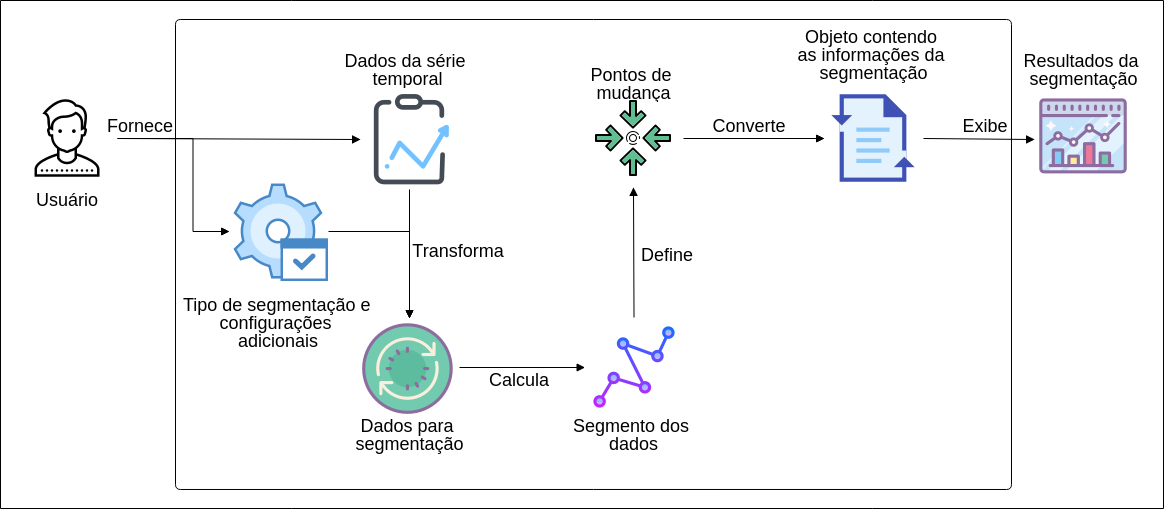
\includegraphics[width=1\textwidth]{./dados/figuras/metodologia-tcc}
    \fonte{Autoria Própria}
    \label{fig:metodologia-tcc}
\end{figure}

O procedimento de escolha de algoritmos é representado na (Figura 6), de forma a exemplificar o modelo de seleção a ser usado como base no desenvolvimento do projeto. Os métodos de segmentação de entrada serão escolhidos por meio de parâmetros na função de segmentação, assim podendo ser identificado qual método escolhido e quais atributos adicionais serão inseridos referente ao modelo de segmentação selecionado. 

A partir da segmentação a saída dos resultados serão padronizadas contendo os dados de entrada, os resultados dos cálculos e informações referentes a chamada da função, descrevendo quais os parâmetros utilizados no cálculo dos pontos de mudança. Portanto, com o objeto retornado será possível plotar gráficos de acordo com o desejo do usuário, ao usar a função de plotar da linguagem R. 

\section{BASE DE DADOS} 
\label{sec:baseDeDados} 

Para testar o desempenho do algoritmo criado, os dados do Coriell \cite{Snijders2001} será utilizado, utilizando as linhas celulares disponibilizadas pelo projeto. Esses dados são utilizados em vários projetos similares, como o DNAcopy \cite{Olshen2004} e \cite{Girimurugan2018}. 

A base de dados disponibilizadas como Coriell possui informações relevantes sobre a linha celular, como o clone que as informações foram tiradas, o cromossomo de referência, a sua variação e assim por diante. A estrutura presente nas informações disponibilizadas do coriell é semelhante a \autoref{tab:tabela-2-dados}, onde são apresentadas os cinco primeiros elementos referente a linha celular do GM05296 e GM13330, dispostas pelo Coriell \cite{Snijders2001}. 

% ######## init table ########
\begin{table}[h]
 \centering
% distancia entre a linha e o texto
 {\renewcommand\arraystretch{1.25}
 \caption{Cinco primeiros dados do Coriell correspondentes a amostra GM05296 e GM13330 contidos na base do DNAcopy}
 \label{tab:tabela-2-dados}
 \begin{tabular}{ l l l l l }
  \cline{1-1}\cline{2-2}\cline{3-3}\cline{4-4}\cline{5-5}  
    \multicolumn{1}{c}{Clone \centering } &
    \multicolumn{1}{c}{Chromosome \centering } &
    \multicolumn{1}{c}{Position \centering } &
    \multicolumn{1}{c}{Coriell.05296 \centering } &
    \multicolumn{1}{c}{Coriell.13330 \centering }
  \\  
  \cline{1-1}\cline{2-2}\cline{3-3}\cline{4-4}\cline{5-5}  
    \multicolumn{1}{c}{GS1-232B23 \centering } &
    \multicolumn{1}{c}{1 \centering } &
    \multicolumn{1}{c}{0 \centering } &
    \multicolumn{1}{c}{NA \centering } &
    \multicolumn{1}{c}{0.207470 \centering }
  \\  
  \cline{1-1}\cline{2-2}\cline{3-3}\cline{4-4}\cline{5-5}  
    \multicolumn{1}{c}{RP11-82d16 \centering } &
    \multicolumn{1}{c}{1 \centering } &
    \multicolumn{1}{c}{468 \centering } &
    \multicolumn{1}{c}{0.008824 \centering } &
    \multicolumn{1}{c}{0.063076 \centering }
  \\  
  \cline{1-1}\cline{2-2}\cline{3-3}\cline{4-4}\cline{5-5}  
    \multicolumn{1}{c}{RP11-62m23 \centering } &
    \multicolumn{1}{c}{1 \centering } &
    \multicolumn{1}{c}{2241 \centering } &
    \multicolumn{1}{c}{-0.000890 \centering } &
    \multicolumn{1}{c}{0.123881 \centering }
  \\  
  \cline{1-1}\cline{2-2}\cline{3-3}\cline{4-4}\cline{5-5}  
    \multicolumn{1}{c}{RP11-60j11 \centering } &
    \multicolumn{1}{c}{1 \centering } &
    \multicolumn{1}{c}{4504 \centering } &
    \multicolumn{1}{c}{0.075875 \centering } &
    \multicolumn{1}{c}{0.154343 \centering }
  \\  
  \cline{1-1}\cline{2-2}\cline{3-3}\cline{4-4}\cline{5-5}  
    \multicolumn{1}{c}{RP11-111O05 \centering } &
    \multicolumn{1}{c}{1 \centering } &
    \multicolumn{1}{c}{5440 \centering } &
    \multicolumn{1}{c}{0.017303 \centering } &
    \multicolumn{1}{c}{-0.043890 \centering }
  \\  
  \hline

 \end{tabular} }
 \fonte{Autoria Própria}
\end{table} 

\section{VALIDAÇÃO} 

O método proposto necessitará ser validado para que haja uma garantia de que os pontos de mudanças sejam conservados no mesmo local, assim obtendo uma maior veracidade na confiança do trabalho desenvolvido. Portanto, para garantir efetividade do algoritmo será utilizado a Matriz de Confusão aplicada aos dados descritos na \autoref{sec:baseDeDados} para obter uma análise do desempenho do algoritmo.